\section{Task 1: Program Development}
\label{sec:task1}

\subsection{Objective}
The objective of Task 1 is to develop a full Newton-Raphson load-flow program from first principles for the IEEE 9-bus system. The final code file is \texttt{E21345\_LoadFlow.py}, which reads input from \texttt{IEEE9\_Bus\_system\_data.json}, constructs the network admittance matrix in code, performs iterative NR solution, and reports voltages, mismatches, line flows, and system losses.

\subsection{Input Data Approach}
Power-flow programs can read data from several sources such as inline/manual input, text files, CSV files, or JSON files. In this work, JSON was selected because it provides structured key-value storage for buses, generators, transformers, lines, and loads in a readable format. The code still follows the assignment requirement of directly accepting text-file-based input.

\begin{table}[H]
  \centering
  \caption{Input dataset summary (from \texttt{IEEE9\_Bus\_system\_data.json}).}
  \label{tab:task1_input_summary}
  \begin{tabular}{lc}
    \toprule
    Data block & Count \\
    \midrule
    Buses & 9 \\
    Generators & 3 \\
    Transformers & 3 \\
    Transmission lines & 6 \\
    Load buses & 3 \\
    Base power & 100 MVA \\
    \bottomrule
  \end{tabular}
\end{table}

\subsection{Mathematical Formulation}
The polar-form power-flow equations are solved using Newton-Raphson \cite{tinney1967powerflow,grainger1994power,saadat1999power}:
\begin{align}
P_i &= \sum_{k=1}^{n} |V_i||V_k|\left(G_{ik}\cos\theta_{ik} + B_{ik}\sin\theta_{ik}\right), \\
Q_i &= \sum_{k=1}^{n} |V_i||V_k|\left(G_{ik}\sin\theta_{ik} - B_{ik}\cos\theta_{ik}\right).
\end{align}
The mismatch vector and update are:
\begin{equation}
\Delta \mathbf{f} =
\begin{bmatrix}
\Delta \mathbf{P} \\
\Delta \mathbf{Q}
\end{bmatrix},
\qquad
\mathbf{J}\Delta\mathbf{x} = \Delta\mathbf{f},
\qquad
\mathbf{x}^{(k+1)} = \mathbf{x}^{(k)} + \Delta\mathbf{x},
\end{equation}
with Jacobian partition
\begin{equation}
\mathbf{J}=
\begin{bmatrix}
J_1 & J_2 \\
J_3 & J_4
\end{bmatrix}.
\end{equation}

Model settings used in code:
\begin{itemize}
  \item Slack bus: 1
  \item PV buses: 2, 3
  \item PQ buses: 4, 5, 6, 7, 8, 9
  \item Flat start: all unknown \(|V|=1.0\) p.u., all angles \(=0^\circ\)
  \item Convergence tolerance: \(10^{-4}\) p.u. mismatch
\end{itemize}

\subsection{Program Flowcharts with Line References}
The assignment asks for flowcharts with line references. Figures~\ref{fig:project_flow}, \ref{fig:task1_code_flow}, and \ref{fig:task1_nr_flow} are the exported flowcharts corresponding to the final script.

\begin{figure}[H]
  \centering
  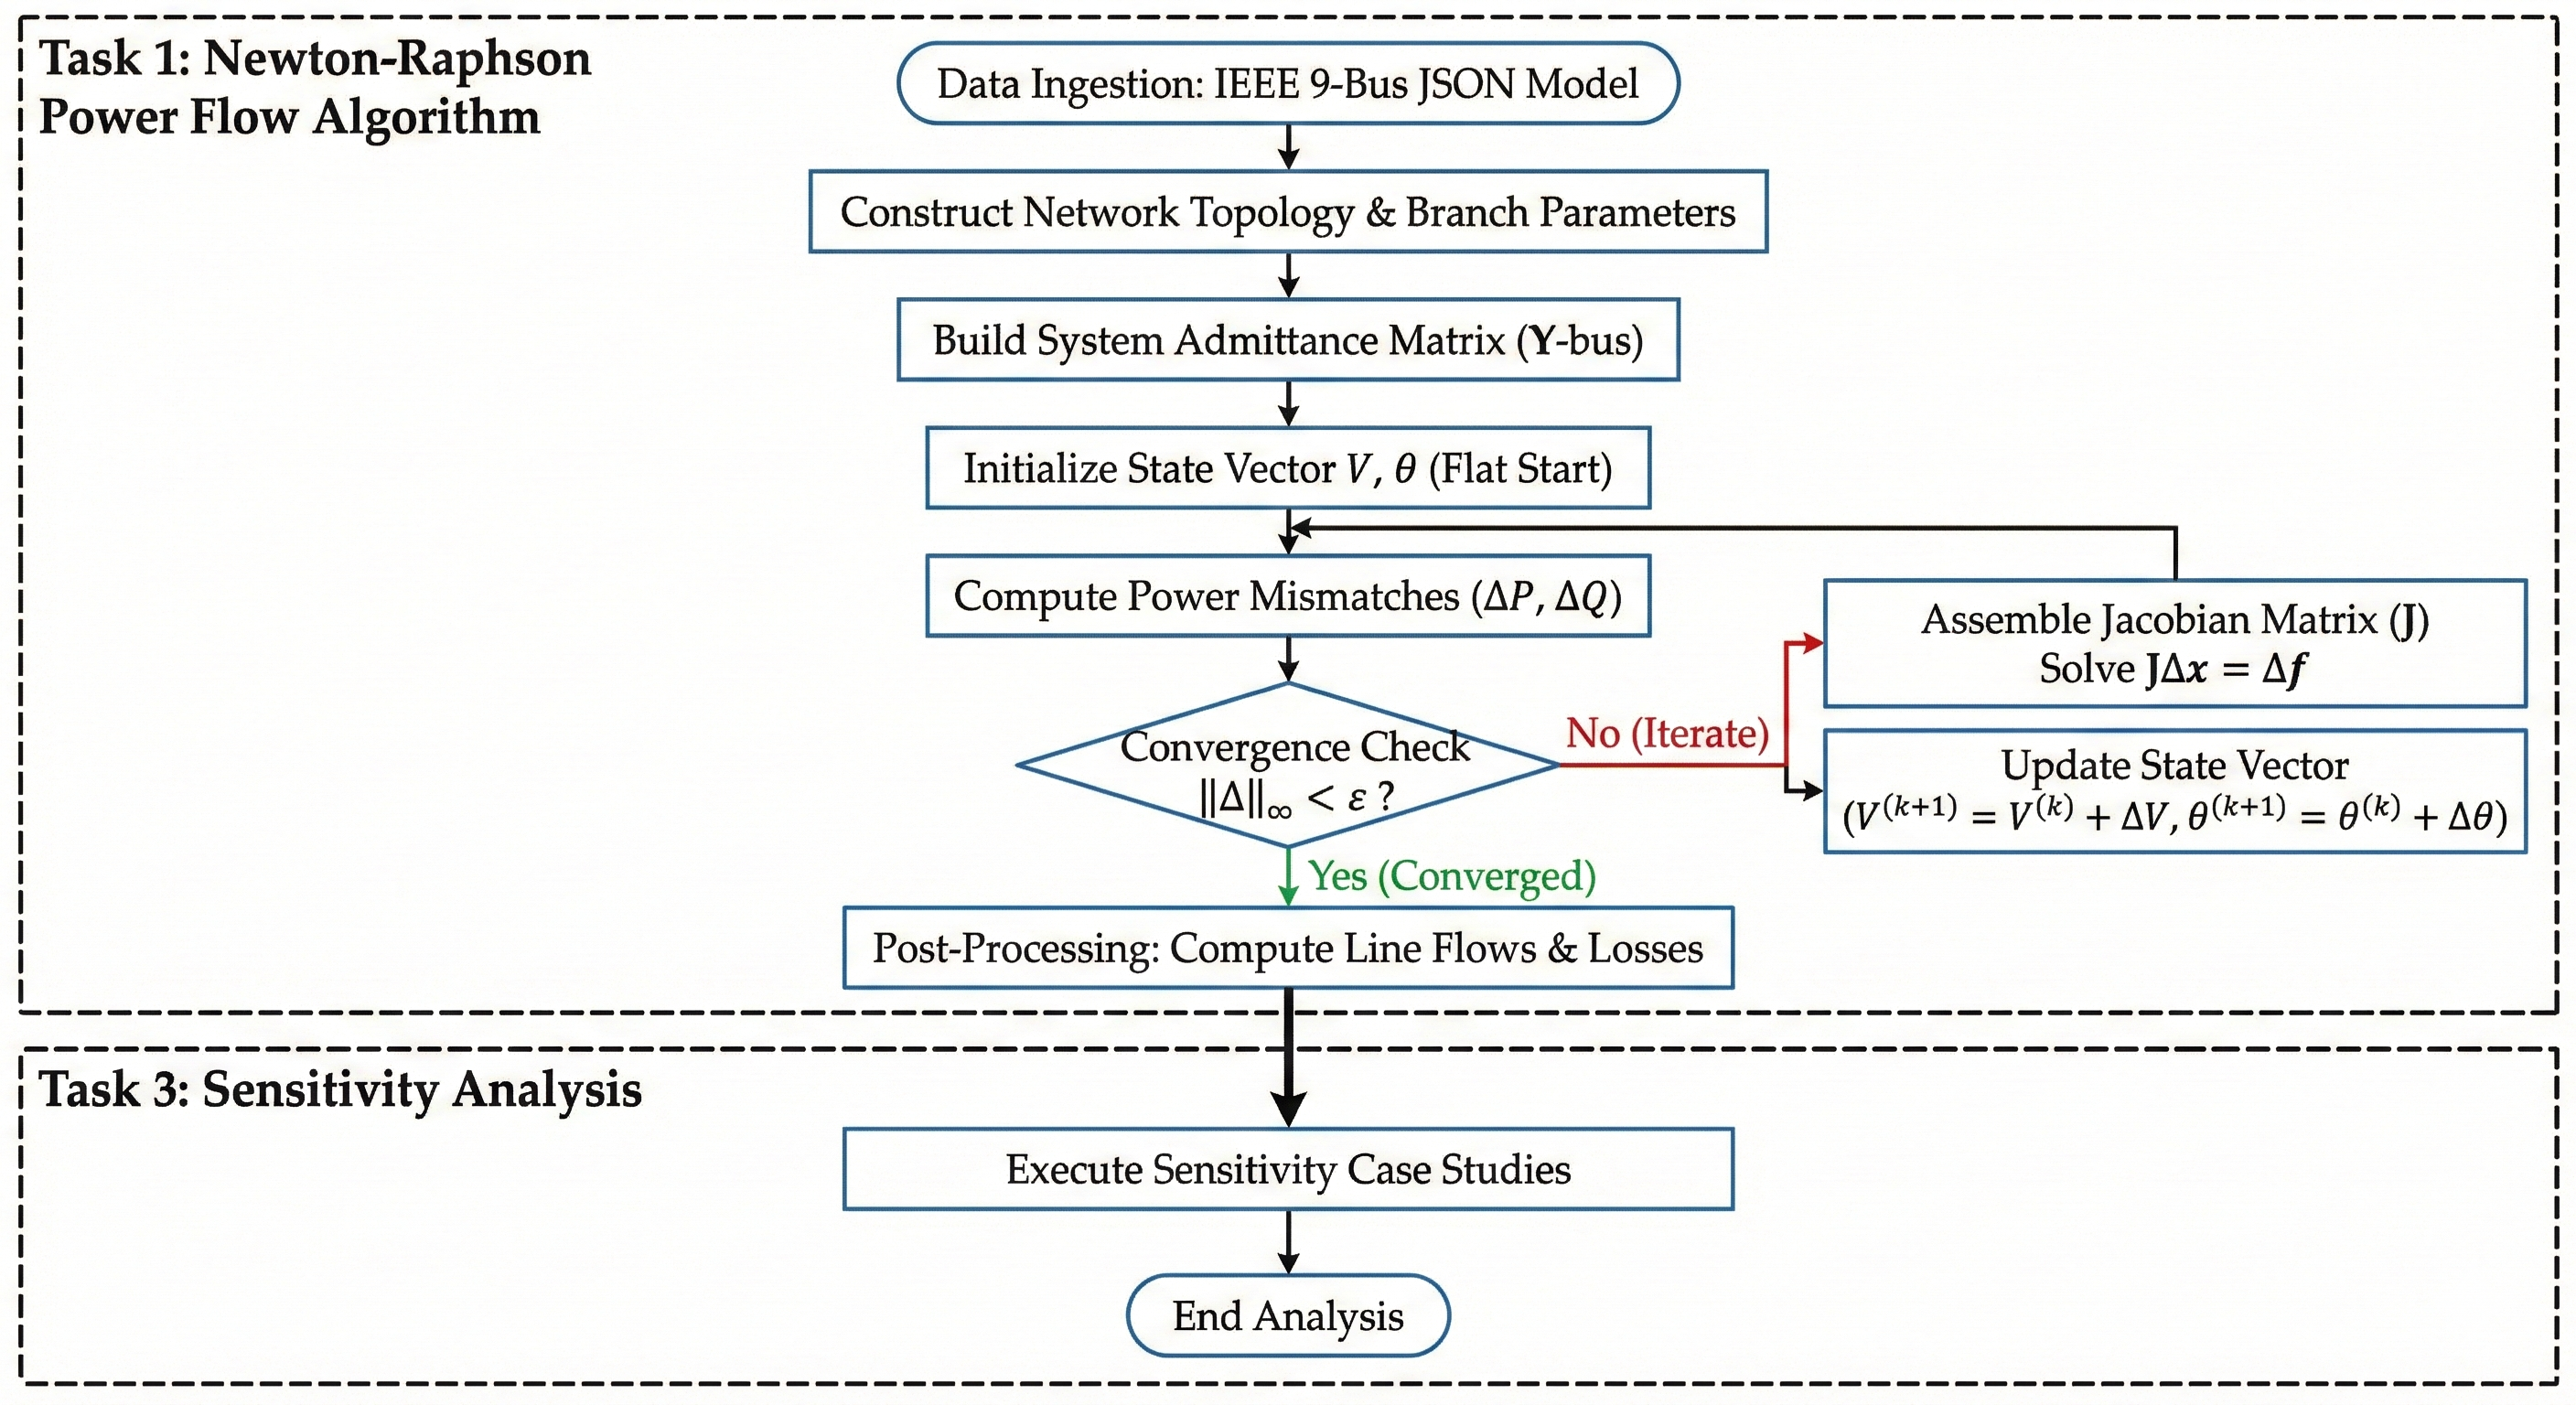
\includegraphics[width=0.92\linewidth]{\detokenize{Figures/Project Flow.png}}
  \caption{Overall project workflow used to organize Tasks 1--3.}
  \label{fig:project_flow}
\end{figure}

\begin{figure}[H]
  \centering
  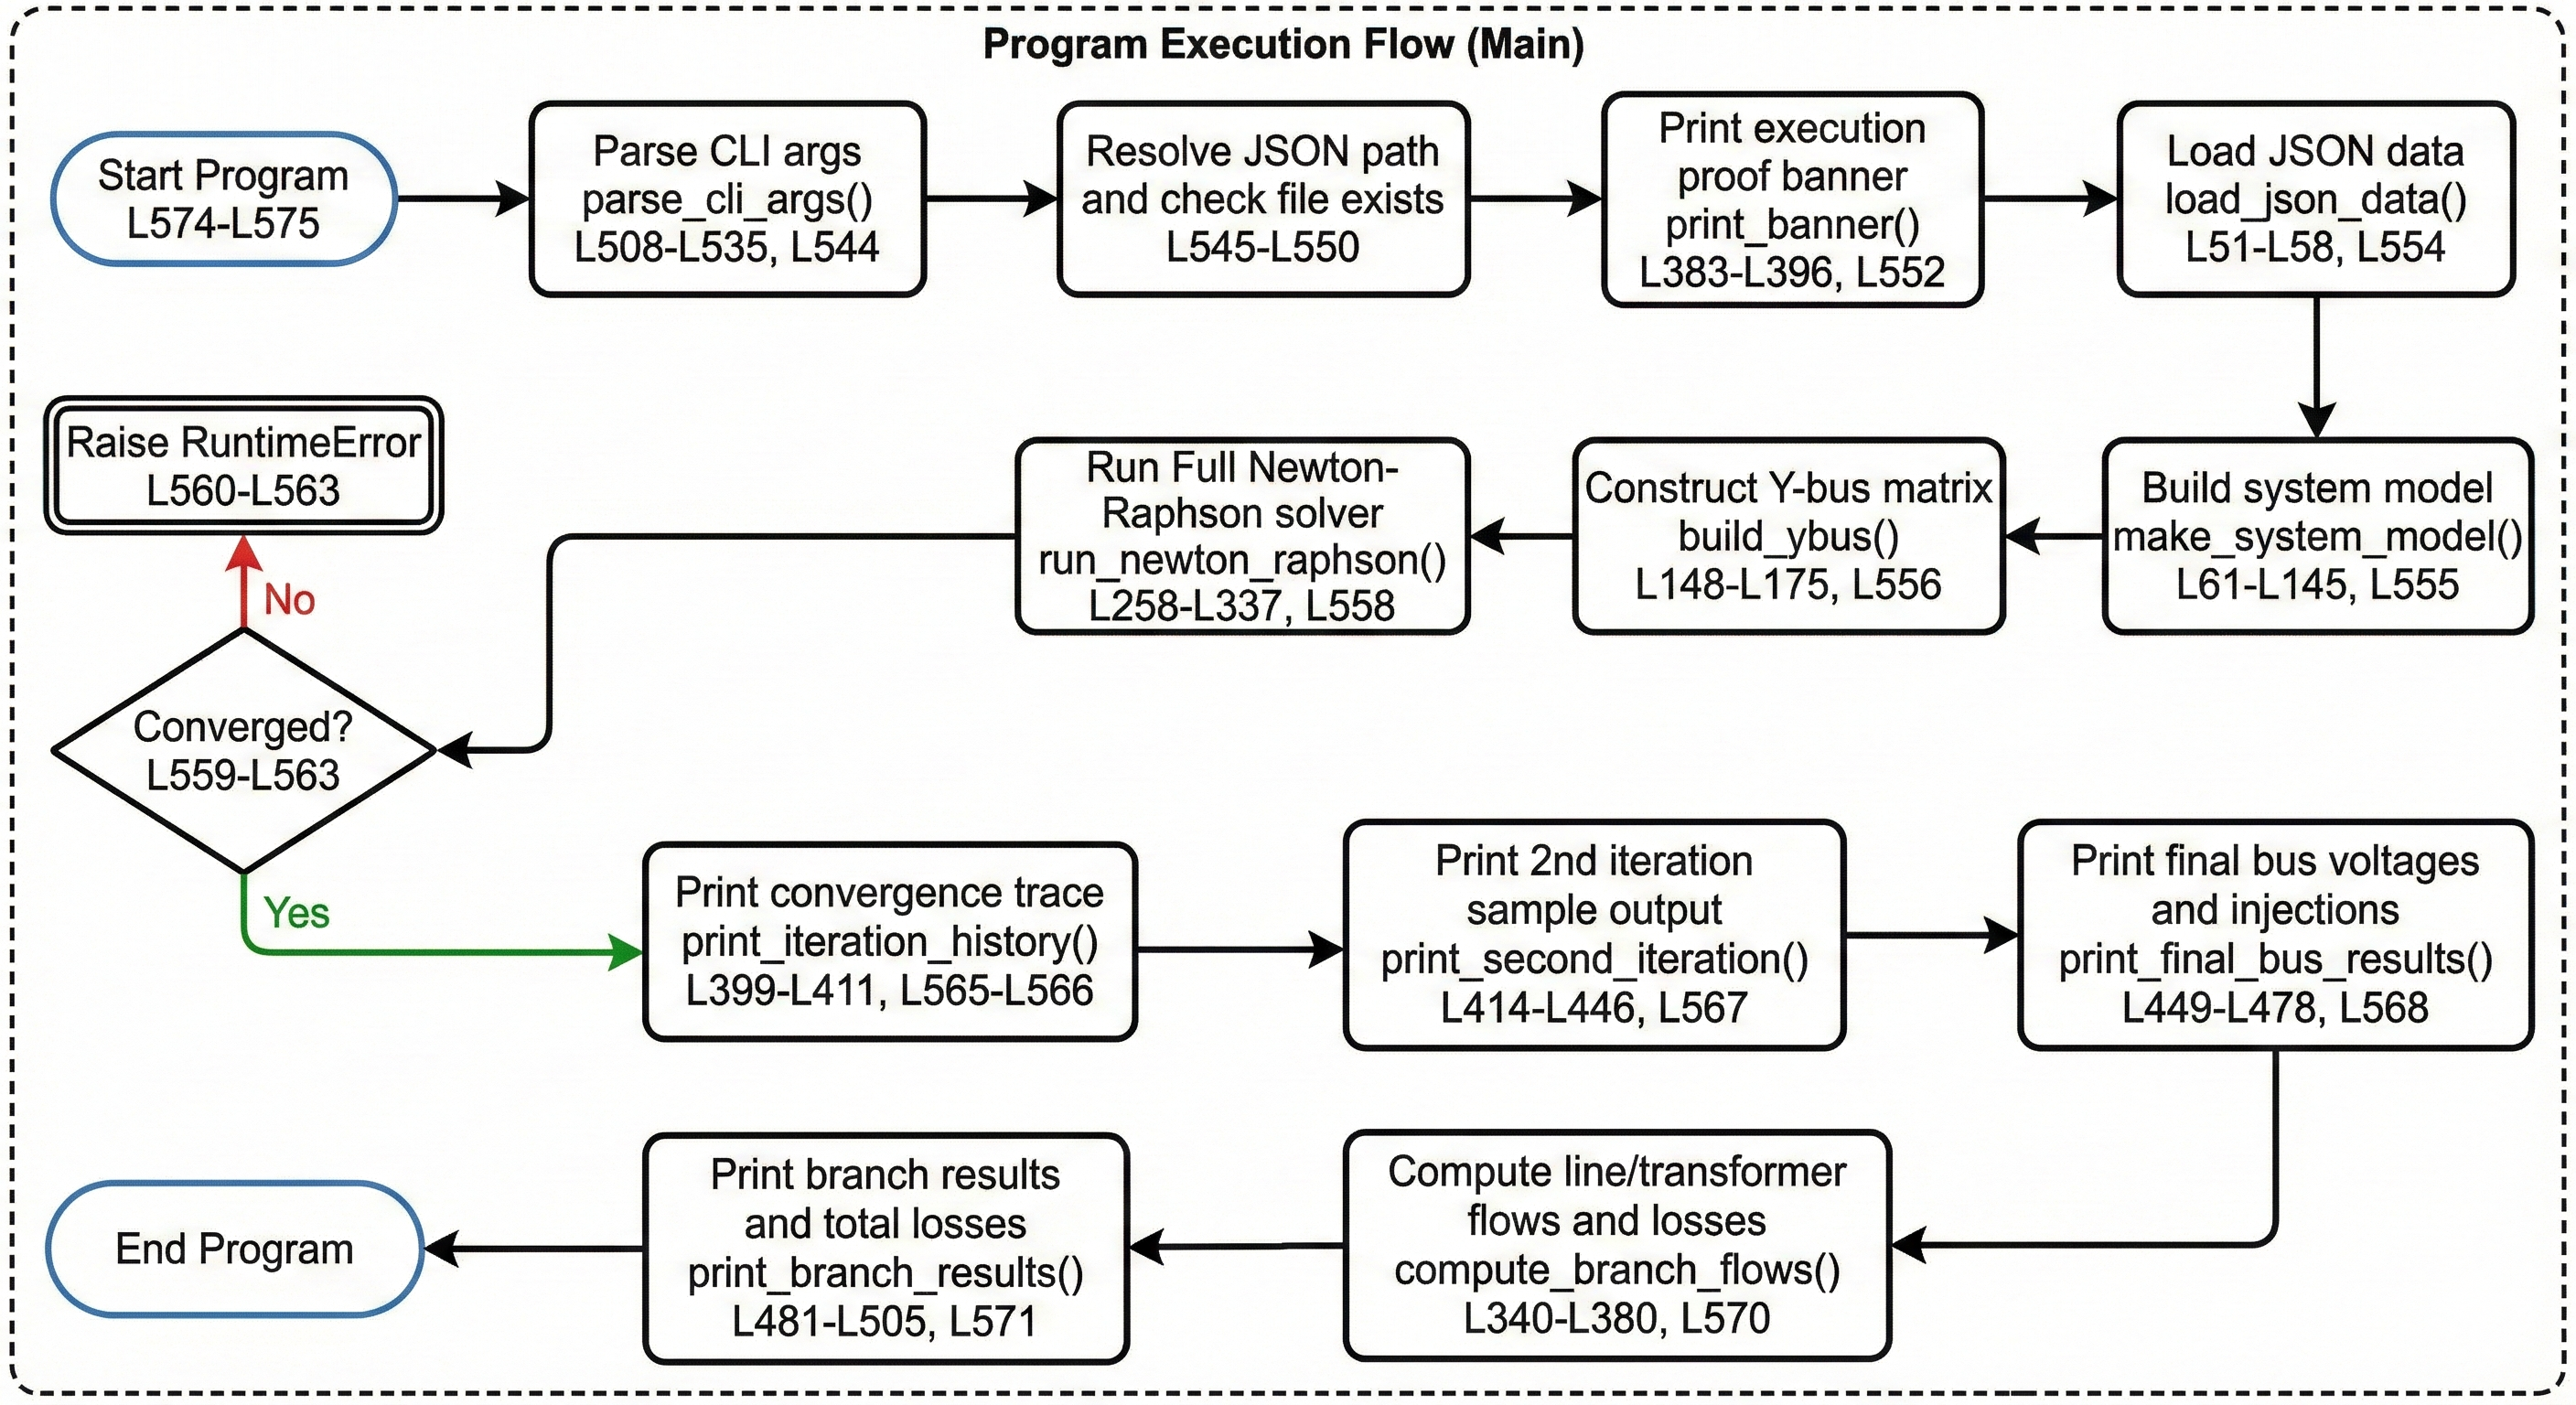
\includegraphics[width=0.95\linewidth]{\detokenize{Figures/task01_Code Flow Chart.png}}
  \caption{Task 1 source-code flowchart linked to \texttt{E21345\_LoadFlow.py} line ranges.}
  \label{fig:task1_code_flow}
\end{figure}

\begin{figure}[H]
  \centering
  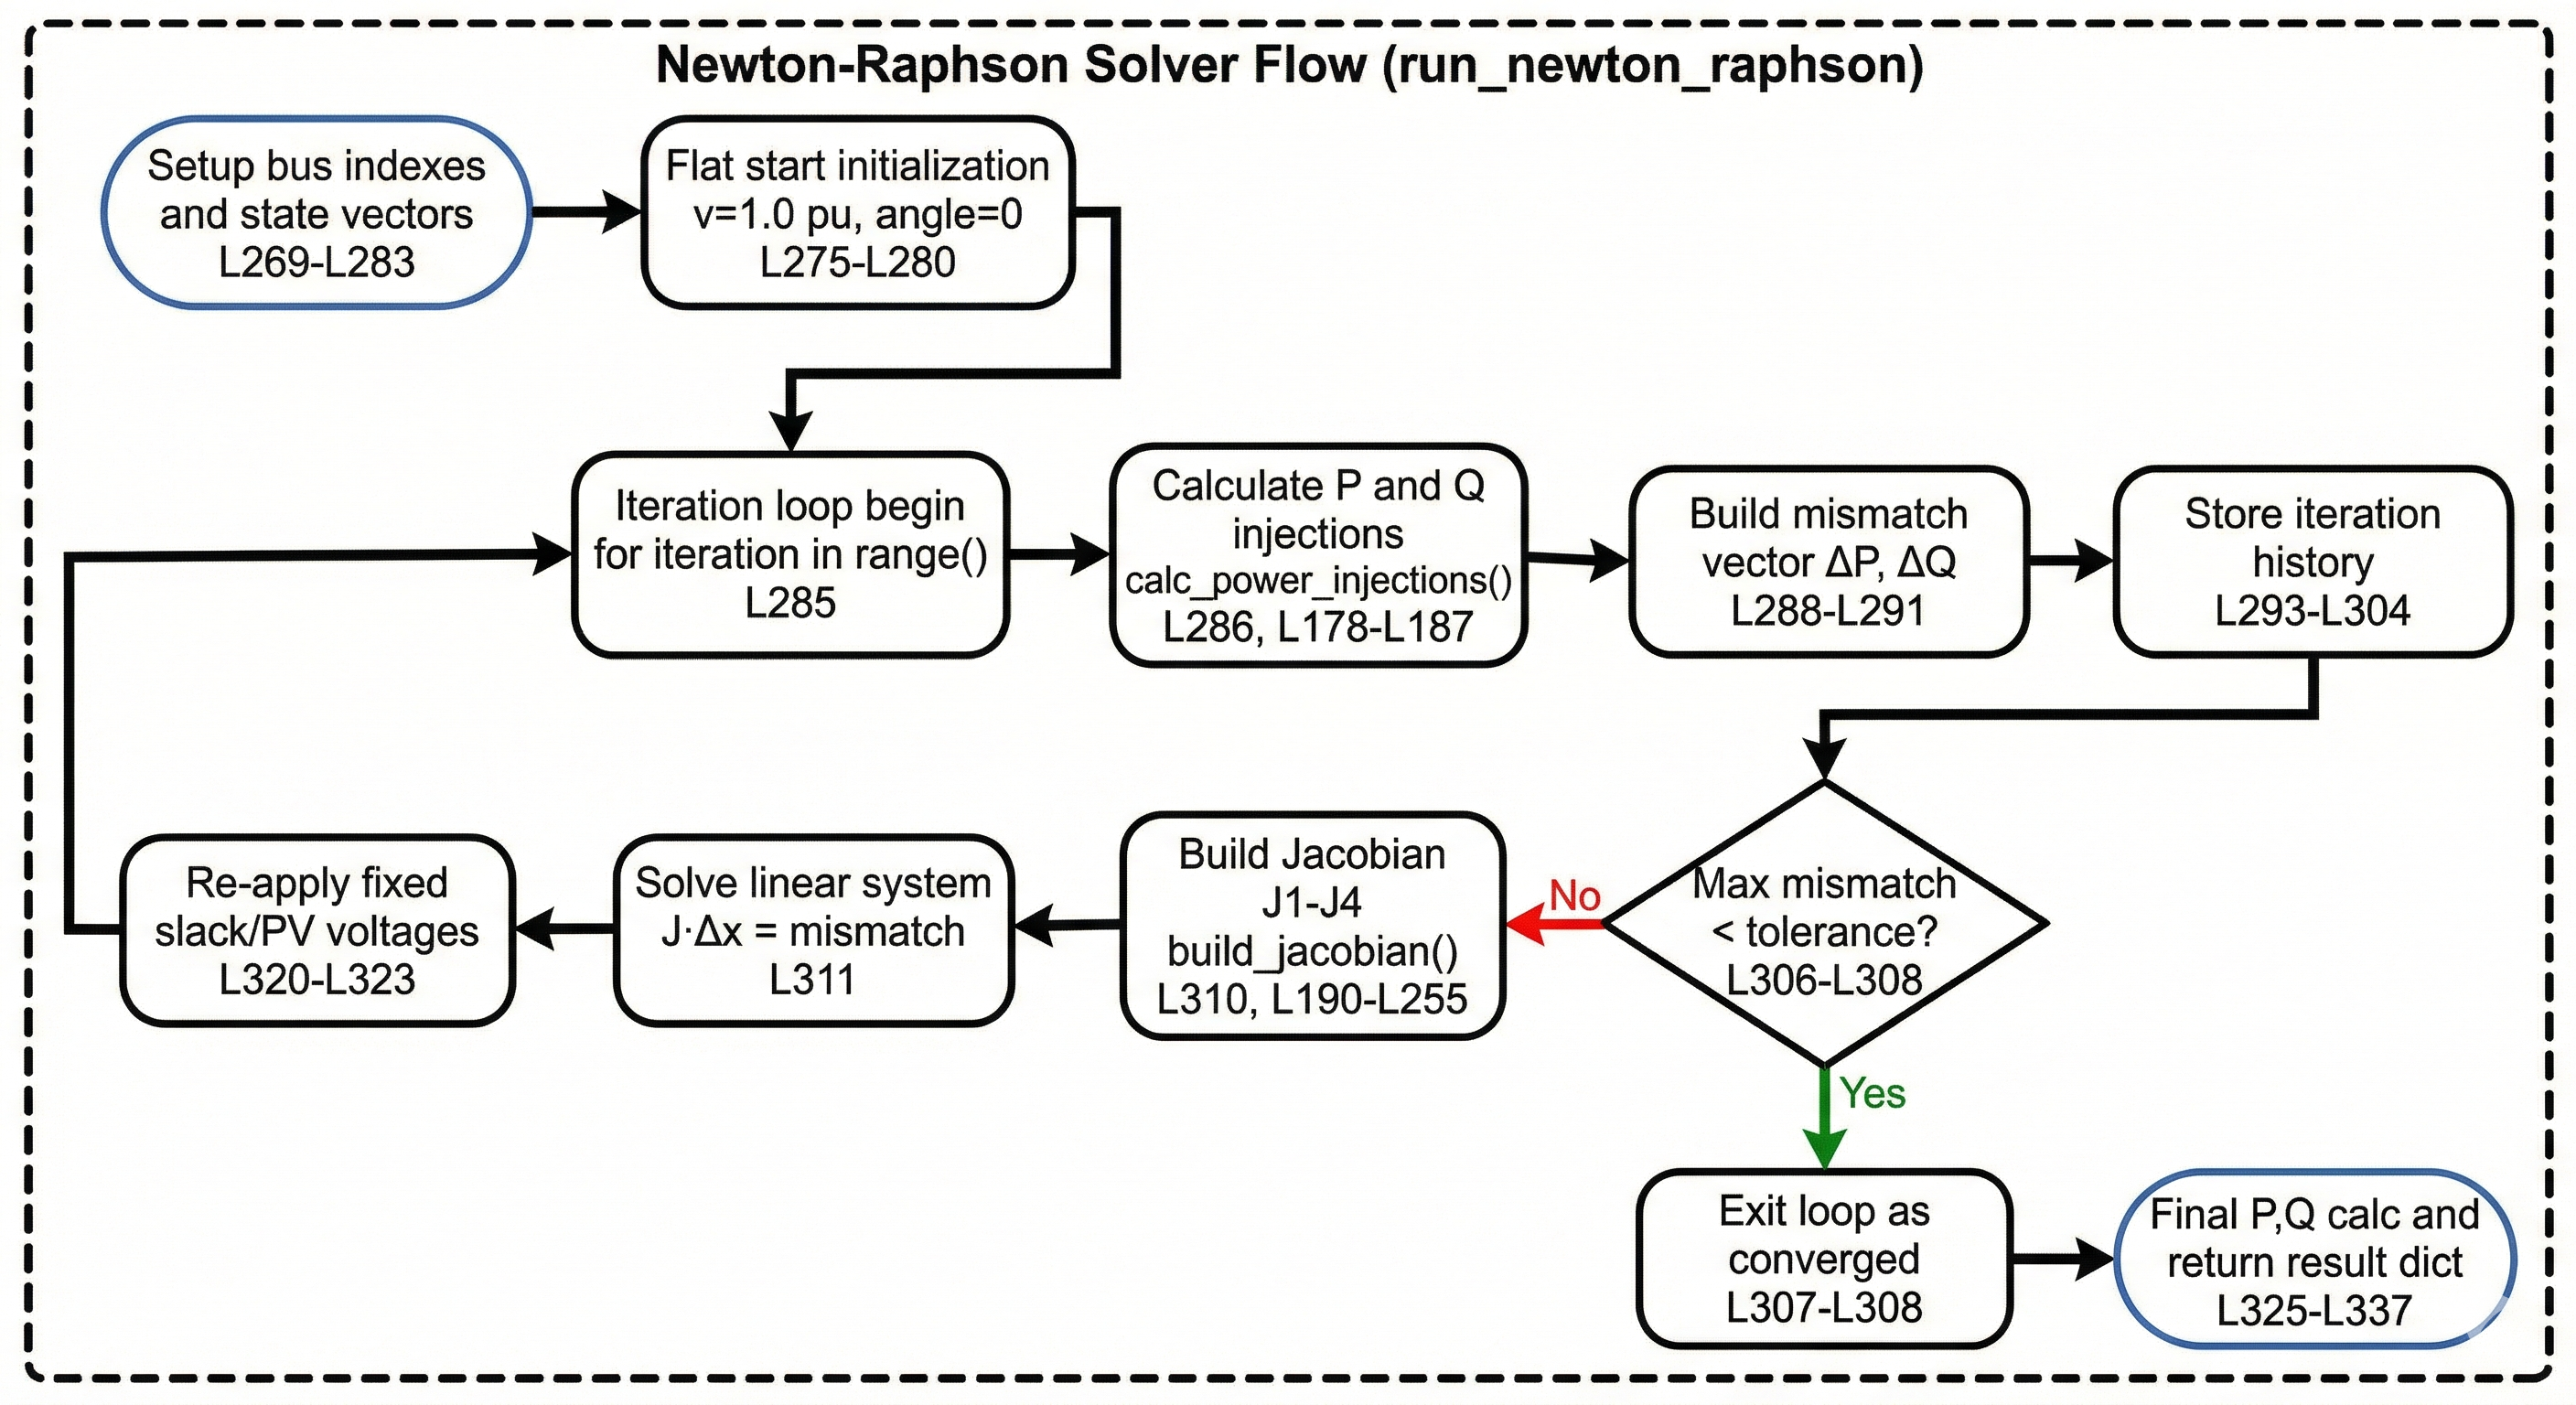
\includegraphics[width=0.95\linewidth]{\detokenize{Figures/task01_NR Function Flow Chart.png}}
  \caption{Newton-Raphson internal function flowchart (mismatch, Jacobian, correction loop).}
  \label{fig:task1_nr_flow}
\end{figure}

\subsection{Y-bus Matrix from Code}
The Y-bus matrix is built directly from line/transformer data in code (no hand calculation).  
The real and imaginary parts are shown in Tables~\ref{tab:ybus_real} and \ref{tab:ybus_imag}.

\begin{table}[H]
\centering
\caption{Real part of \(Y_{bus}\) (p.u.).}
\label{tab:ybus_real}
\scriptsize
\resizebox{\textwidth}{!}{
\begin{tabular}{c|rrrrrrrrr}
\toprule
Bus & 1 & 2 & 3 & 4 & 5 & 6 & 7 & 8 & 9 \\
\midrule
1 & 0.00000 & 0.00000 & 0.00000 & 0.00000 & 0.00000 & 0.00000 & 0.00000 & 0.00000 & 0.00000 \\
2 & 0.00000 & 0.00000 & 0.00000 & 0.00000 & 0.00000 & 0.00000 & 0.00000 & 0.00000 & 0.00000 \\
3 & 0.00000 & 0.00000 & 0.00000 & 0.00000 & 0.00000 & 0.00000 & 0.00000 & 0.00000 & 0.00000 \\
4 & 0.00000 & 0.00000 & 0.00000 & 3.30738 & -1.36519 & -1.94219 & 0.00000 & 0.00000 & 0.00000 \\
5 & 0.00000 & 0.00000 & 0.00000 & -1.36519 & 2.55279 & 0.00000 & -1.18760 & 0.00000 & 0.00000 \\
6 & 0.00000 & 0.00000 & 0.00000 & -1.94219 & 0.00000 & 3.22420 & 0.00000 & 0.00000 & -1.28201 \\
7 & 0.00000 & 0.00000 & 0.00000 & 0.00000 & -1.18760 & 0.00000 & 2.80473 & -1.61712 & 0.00000 \\
8 & 0.00000 & 0.00000 & 0.00000 & 0.00000 & 0.00000 & 0.00000 & -1.61712 & 2.77221 & -1.15509 \\
9 & 0.00000 & 0.00000 & 0.00000 & 0.00000 & 0.00000 & -1.28201 & 0.00000 & -1.15509 & 2.43710 \\
\bottomrule
\end{tabular}}
\normalsize
\end{table}

\begin{table}[H]
\centering
\caption{Imaginary part of \(Y_{bus}\) (p.u.).}
\label{tab:ybus_imag}
\scriptsize
\resizebox{\textwidth}{!}{
\begin{tabular}{c|rrrrrrrrr}
\toprule
Bus & 1 & 2 & 3 & 4 & 5 & 6 & 7 & 8 & 9 \\
\midrule
1 & -17.36111 & 0.00000 & 0.00000 & 17.36111 & 0.00000 & 0.00000 & 0.00000 & 0.00000 & 0.00000 \\
2 & 0.00000 & -16.00000 & 0.00000 & 0.00000 & 0.00000 & 0.00000 & 16.00000 & 0.00000 & 0.00000 \\
3 & 0.00000 & 0.00000 & -17.06485 & 0.00000 & 0.00000 & 0.00000 & 0.00000 & 0.00000 & 17.06485 \\
4 & 17.36111 & 0.00000 & 0.00000 & -39.30889 & 11.60410 & 10.51068 & 0.00000 & 0.00000 & 0.00000 \\
5 & 0.00000 & 0.00000 & 0.00000 & 11.60410 & -17.33823 & 0.00000 & 5.97513 & 0.00000 & 0.00000 \\
6 & 0.00000 & 0.00000 & 0.00000 & 10.51068 & 0.00000 & -15.84093 & 0.00000 & 0.00000 & 5.58824 \\
7 & 0.00000 & 16.00000 & 0.00000 & 0.00000 & 5.97513 & 0.00000 & -35.44561 & 13.69798 & 0.00000 \\
8 & 0.00000 & 0.00000 & 0.00000 & 0.00000 & 0.00000 & 0.00000 & 13.69798 & -23.30325 & 9.78427 \\
9 & 0.00000 & 0.00000 & 17.06485 & 0.00000 & 0.00000 & 5.58824 & 0.00000 & 9.78427 & -32.15386 \\
\bottomrule
\end{tabular}}
\normalsize
\end{table}

\subsection{Convergence and Sample Iteration Output}
\begin{table}[H]
  \centering
  \caption{Task 1 convergence summary for IEEE 9-bus base case.}
  \label{tab:task1_conv}
  \begin{tabular}{lc}
    \toprule
    Item & Value \\
    \midrule
    Tolerance & \(10^{-4}\) p.u. \\
    Total iterations to convergence & 4 \\
    Total active power loss & 4.641023 MW \\
    Total reactive power loss & -92.160126 MVAr \\
    \bottomrule
  \end{tabular}
\end{table}

\begin{table}[H]
  \centering
  \caption{Second-iteration bus snapshot (assignment deliverable).}
  \label{tab:task1_iter2}
  \scriptsize
  \begin{tabular}{ccccc}
    \toprule
    Bus & \(|V|_{iter2}\) (p.u.) & \(\theta_{iter2}\) (deg) & \(P_{calc}\) (p.u.) & \(Q_{calc}\) (p.u.) \\
    \midrule
    1 & 1.040000 & 0.000000 & 0.692229 & 0.131738 \\
    2 & 1.025000 & 9.891070 & 1.687927 & -0.116864 \\
    3 & 1.025000 & 5.199844 & 0.883627 & -0.240382 \\
    4 & 1.033415 & -2.126114 & 0.010614 & 0.050091 \\
    5 & 1.008445 & -3.828628 & -1.287904 & -0.428586 \\
    6 & 1.022349 & -3.595802 & -0.943938 & -0.257555 \\
    7 & 1.037245 & 4.196429 & 0.042054 & 0.187516 \\
    8 & 1.026641 & 1.093843 & -1.061005 & -0.325875 \\
    9 & 1.039970 & 2.415549 & 0.026887 & 0.082844 \\
    \bottomrule
  \end{tabular}
  \normalsize
\end{table}

\begin{table}[H]
  \centering
  \caption{Final bus voltage profile from custom NR solver.}
  \label{tab:task1_finalV}
  \begin{tabular}{ccc}
    \toprule
    Bus & \(|V|\) (p.u.) & Angle (deg) \\
    \midrule
    1 & 1.040000 & 0.000000 \\
    2 & 1.025000 & 9.280008 \\
    3 & 1.025000 & 4.664753 \\
    4 & 1.025788 & -2.216787 \\
    5 & 0.995631 & -3.988804 \\
    6 & 1.012654 & -3.687395 \\
    7 & 1.025769 & 3.719704 \\
    8 & 1.015883 & 0.727538 \\
    9 & 1.032353 & 1.966718 \\
    \bottomrule
  \end{tabular}
\end{table}

\begin{table}[H]
  \centering
  \caption{Line/transformer power flows and branch losses from custom NR run.}
  \label{tab:task1_flows}
  \scriptsize
  \begin{tabular}{lrrrrrr}
    \toprule
    Branch & \(P_{i\to j}\) MW & \(Q_{i\to j}\) MVAr & \(P_{j\to i}\) MW & \(Q_{j\to i}\) MVAr & \(P_{loss}\) MW & \(Q_{loss}\) MVAr \\
    \midrule
    T(1-4) & 71.6410 & 27.0459 & -71.6410 & -23.9231 & 0.0000 & 3.1228 \\
    T(2-7) & 163.0000 & 6.6536 & -163.0000 & 9.1782 & 0.0000 & 15.8318 \\
    T(3-9) & 85.0000 & -10.8597 & -85.0000 & 14.9554 & 0.0000 & 4.0956 \\
    L(4-5) & 40.9373 & 22.8931 & -40.6798 & -38.6872 & 0.2575 & -15.7941 \\
    L(4-6) & 30.7037 & 1.0300 & -30.5373 & -16.5434 & 0.1664 & -15.5134 \\
    L(5-7) & -84.3202 & -11.3127 & 86.6202 & -8.3808 & 2.3000 & -19.6936 \\
    L(6-9) & -59.4628 & -13.4566 & 60.8166 & -18.0748 & 1.3538 & -31.5315 \\
    L(7-8) & 76.3799 & -0.7973 & -75.9046 & -10.7042 & 0.4753 & -11.5015 \\
    L(8-9) & -24.0954 & -24.2958 & 24.1834 & 3.1195 & 0.0880 & -21.1763 \\
    \bottomrule
  \end{tabular}
  \normalsize
\end{table}

\subsection{Execution Proof Requirement}
The source code prints student identification and timestamp at runtime:
\begin{itemize}
  \item \texttt{Student Name: Samarakoon S.M.O.T.}
  \item \texttt{Student ID: E/21/345}
  \item \texttt{Run Timestamp: YYYY-MM-DD HH:MM:SS}
\end{itemize}
This directly supports the required submission screenshot condition.

\subsection{Task 1 Discussion}
The custom NR solver converged in four iterations with monotonic mismatch reduction. The solved operating point and branch-flow pattern are consistent with textbook IEEE 9-bus behavior and with expected NR convergence properties \cite{tinney1967powerflow,saadat1999power,chapman2011electric}. The transformer branches carry no active loss due zero resistance assumptions in the provided dataset, while transmission lines account for the net active losses. The obtained loss level (about 4.64 MW) is reasonable for this loading pattern and network parameters.

